
\clearpage


\section*{Appendix}

\section{Detailed Results on MMEB-V2}

We report detailed results of \ours{} and strong baselines on MMEB-V2, which contains 78 tasks spanning three modality groups: \textbf{Image}, \textbf{Video}, and \textbf{Visual Document} (VisDoc).
Table~\ref{tab:full_score_image} summarizes overall performance and provides a breakdown of the \textbf{Image} group (36 tasks; Hit@1), including both meta-task averages and per-dataset results.
Table~\ref{tab:full_score_video} presents detailed \textbf{Video} results (18 tasks; Hit@1).
Table~\ref{tab:full_score_visdoc} reports detailed \textbf{VisDoc} results (24 tasks; NDCG@5), covering document-level retrieval benchmarks such as ViDoRe.
For readability and to fit the appendix layout, we split the detailed results into three tables.




\definecolor{avgcolor}{RGB}{242,248,236}     % light green
\definecolor{icatcolor}{RGB}{255,243,233}    % light peach
\definecolor{vcatcolor}{RGB}{235,248,255}    % light cyan
\definecolor{vdcatcolor}{RGB}{250,236,244}   % light pink


\begin{table*}[!t]
    \centering
\caption{Detailed results on the full MMEB-v2 benchmark: summary and image tasks (36 tasks, Hit@1).}
\label{tab:full_score_image}
    \renewcommand{\arraystretch}{1.1}
    \begin{adjustbox}{width=\textwidth}
    \begin{tabular}{l|ccccccccc}
        \toprule
        ~ & GME & VLM2Vec-v1 & VLM2Vec-v2 & CAFe & UME-R1 & LCO-EMB & Omni-Embed-Nemotron & \ours{} & \ours{} \\
        Model Size & 7B & 7B & 2B & 7B & 7B & 7B & 3B & 3B & 7B \\
        \midrule
        \rowcolor{avgcolor}
        Avg - All (78 tasks) & 57.8 & 52.3 & 58.0 & 60.6 & 64.5 & 50.6 & 51.5 & 63.1 & 66.4 \\
        \rowcolor{avgcolor}
        Avg - Image (36 tasks, Hit@1) & 56.0 & 65.5 & 64.9 & 67.6 & 71.3 & 44.0 & 43.7 & 67.6 & 71.2 \\
        \rowcolor{avgcolor}
        Avg - Video (18 tasks, Hit@1) & 38.4 & 33.7 & 34.6 & 42.4 & 47.5 & 38.2 & 36.9 & 40.6 & 43.5 \\
        \rowcolor{avgcolor}
        Avg - Visdoc (24 tasks, NDCG@5) & 75.2 & 46.4 & 65.4 & 63.9 & 67.1 & 69.8 & 74.2 & 73.2 & 76.1 \\
        \rowcolor{icatcolor}
        I-CLS (10) & 57.7 & 62.7 & 62.9 & 63.6 & 67.1 & 56.3 & 46.0 & 64.7 & 66.7 \\
        \rowcolor{icatcolor}
        I-QA (10) & 34.7 & 56.9 & 56.3 & 61.7 & 69.2 & 16.9 & 20.5 & 62.1 & 68.5 \\
        \rowcolor{icatcolor}
        I-RET (12) & 71.2 & 69.4 & 69.5 & 69.1 & 71.9 & 52.2 & 58.0 & 70.5 & 73.0 \\
        \rowcolor{icatcolor}
        I-VG (4) & 59.3 & 82.2 & 77.3 & 87.6 & 84.9 & 57.0 & 52.9 & 79.6 & 83.9 \\
        \rowcolor{vcatcolor}
        V-CLS (5) & 37.4 & 39.1 & 39.3 & 35.8 & 48.6 & 39.3 & 40.5 & 40.2 & 46.6 \\
        \rowcolor{vcatcolor}
        V-QA (5) & 50.4 & 30.0 & 34.3 & 58.7 & 60.7 & 57.6 & 44.3 & 48.5 & 52.9 \\
        \rowcolor{vcatcolor}
        V-RET (5) & 28.4 & 29.0 & 28.8 & 34.4 & 38.2 & 24.8 & 32.7 & 33.1 & 36.7 \\
        \rowcolor{vcatcolor}
        V-MR (3) & 37.0 & 38.9 & 36.8 & 39.5 & 39.3 & 26.5 & 25.6 & 40.7 & 34.2 \\
        \rowcolor{vdcatcolor}
        VD-Vidore-V1 (10) & 89.4 & 56.9 & 75.5 & 70.7 & 75.7 & 80.4 & 85.7 & 83.1 & 87.6 \\
        \rowcolor{vdcatcolor}
        VD-Vidore-V2 (4) & 55.6 & 9.4 & 44.9 & 49.6 & 50.5 & 56.4 & 61.3 & 59.5 & 62.4 \\
        \rowcolor{vdcatcolor}
        VD-VisRAG (6) & 85.0 & 59.1 & 79.4 & 79.5 & 83.7 & 79.7 & 84.3 & 85.5 & 87.5 \\
        \rowcolor{vdcatcolor}
        VD-OOD (4) & 44.4 & 38.1 & 39.4 & 38.1 & 37.6 & 41.8 & 43.3 & 43.4 & 44.3 \\
        \midrule
        ImageNet-1K & 64.6 & 80.1 & 80.8 & 77.3 & 80.4 & 73.0 & 57.0 & 76.5 & 79.4 \\
        N24News & 50.5 & 79.7 & 72.9 & 83.2 & 82.3 & 37.5 & 36.4 & 76.7 & 77.2 \\
        HatefulMemes & 53.6 & 69.7 & 56.3 & 78.7 & 79.0 & 45.1 & 48.0 & 66.2 & 72.3 \\
        VOC2007 & 80.3 & 80.7 & 85.0 & 89.8 & 90.8 & 64.9 & 47.9 & 84.8 & 83.9 \\
        SUN397 & 69.5 & 77.4 & 71.0 & 79.9 & 80.3 & 72.0 & 53.1 & 75.1 & 76.1 \\
        Place365 & 39.1 & 37.4 & 35.9 & 45.0 & 46.8 & 40.8 & 30.7 & 41.7 & 44.3 \\
        ImageNet-A & 41.2 & 58.1 & 47.4 & 55.2 & 53.9 & 52.2 & 37.0 & 58.6 & 57.2 \\
        ImageNet-R & 83.9 & 73.9 & 89.3 & 88.0 & 90.1 & 88.9 & 80.9 & 85.5 & 84.5 \\
        ObjectNet & 69.0 & 40.1 & 65.2 & 22.5 & 42.3 & 61.7 & 44.9 & 53.0 & 57.7 \\
        Country211 & 24.8 & 29.8 & 25.2 & 16.7 & 25.0 & 26.5 & 24.1 & 29.1 & 34.7 \\
        OK-VQA & 33.2 & 56.8 & 51.5 & 67.3 & 71.7 & 14.4 & 18.6 & 64.9 & 70.5 \\
        A-OKVQA & 21.0 & 47.3 & 43.6 & 63.8 & 58.7 & 10.9 & 11.9 & 54.8 & 59.7 \\
        DocVQA & 41.4 & 89.7 & 90.1 & 79.2 & 93.8 & 17.5 & 17.3 & 91.2 & 93.3 \\
        InfographicsVQA & 20.3 & 60.0 & 58.8 & 53.3 & 79.2 & 7.4 & 9.1 & 52.8 & 62.9 \\
        ChartQA & 17.8 & 56.9 & 47.4 & 48.8 & 75.1 & 12.7 & 13.1 & 52.7 & 62.8 \\
        Visual7W & 22.2 & 52.7 & 52.9 & 52.5 & 55.2 & 10.8 & 7.4 & 59.8 & 65.2 \\
        ScienceQA & 28.0 & 38.5 & 38.2 & 65.4 & 53.7 & 26.7 & 25.3 & 43.6 & 56.4 \\
        VizWiz & 39.0 & 39.9 & 43.3 & 43.8 & 51.6 & 31.8 & 34.8 & 53.1 & 56.3 \\
        GQA & 76.9 & 55.1 & 64.9 & 65.7 & 69.3 & 11.5 & 31.2 & 65.4 & 72.1 \\
        TextVQA & 46.8 & 71.6 & 72.2 & 76.8 & 83.5 & 25.1 & 36.6 & 82.8 & 86.2 \\
        VisDial & 60.8 & 81.9 & 82.7 & 82.7 & 80.7 & 51.1 & 51.5 & 78.9 & 82.4 \\
        CIRR & 54.9 & 51.1 & 57.5 & 60.4 & 55.3 & 8.4 & 14.8 & 54.9 & 54.9 \\
        VisualNews\_t2i & 79.7 & 80.5 & 74.5 & 69.5 & 76.8 & 61.4 & 58.8 & 74.6 & 75.3 \\
        VisualNews\_i2t & 83.6 & 81.2 & 78.2 & 79.4 & 82.0 & 59.5 & 56.3 & 77.7 & 79.8 \\
        MSCOCO\_t2i & 71.2 & 77.2 & 75.3 & 75.4 & 78.3 & 66.1 & 60.7 & 78.1 & 76.6 \\
        MSCOCO\_i2t & 57.7 & 73.9 & 71.4 & 73.1 & 71.4 & 59.5 & 56.5 & 72.5 & 76.9 \\
        NIGHTS & 67.6 & 67.6 & 68.6 & 66.7 & 68.1 & 65.2 & 65.3 & 68.4 & 68.6 \\
        WebQA & 91.4 & 88.3 & 90.6 & 89.3 & 90.9 & 53.2 & 89.8 & 89.2 & 89.3 \\
        FashionIQ & 37.8 & 17.1 & 19.5 & 39.0 & 23.4 & 3.5 & 6.2 & 19.5 & 24.5 \\
        Wiki-SS-NQ & 78.2 & 62.3 & 66.9 & 61.2 & 72.5 & 64.2 & 87.7 & 74.9 & 79.4 \\
        OVEN & 75.1 & 66.5 & 64.3 & 60.8 & 71.4 & 59.9 & 67.9 & 76.1 & 78.7 \\
        EDIS & 96.0 & 85.7 & 84.1 & 71.3 & 92.0 & 74.4 & 80.5 & 81.7 & 89.6 \\
        MSCOCO & 31.4 & 75.7 & 67.1 & 84.7 & 72.7 & 33.8 & 32.8 & 70.9 & 74.8 \\
        RefCOCO & 60.9 & 87.6 & 87.1 & 89.4 & 91.4 & 50.9 & 59.7 & 85.3 & 89.4 \\
        RefCOCO-Matching & 78.4 & 84.6 & 85.8 & 83.0 & 91.1 & 98.5 & 65.9 & 75.8 & 87.2 \\
        Visual7W-Pointing & 66.5 & 81.0 & 69.2 & 93.2 & 84.2 & 44.6 & 53.1 & 86.5 & 84.3 \\
        \bottomrule
    \end{tabular}
    \end{adjustbox}
\end{table*}

\begin{table*}[!t]
    \centering
\caption{Detailed results on the full MMEB-v2 benchmark: video tasks (18 tasks, Hit@1).}
\label{tab:full_score_video}
    \renewcommand{\arraystretch}{1.1}
    \begin{adjustbox}{width=\textwidth}
    \begin{tabular}{l|ccccccccc}
        \toprule
        ~ & GME & VLM2Vec-v1 & VLM2Vec-v2 & CAFe & UME-R1 & LCO-EMB & Omni-Embed-Nemotron & \ours{} & \ours{} \\
        Model Size & 7B & 7B & 2B & 7B & 7B & 7B & 3B & 3B & 7B \\
        \midrule
        K700 & 39.7 & 35.5 & 38.0 & 40.1 & 42.8 & 40.2 & 36.0 & 41.9 & 48.0 \\
        SmthSmthV2 & 30.6 & 32.1 & 42.8 & 35.8 & 50.4 & 33.3 & 33.4 & 34.4 & 41.3 \\
        HMDB51 & 47.9 & 42.2 & 40.9 & 46.9 & 58.3 & 37.3 & 49.1 & 42.2 & 54.4 \\
        UCF101 & 54.7 & 61.8 & 60.0 & 39.6 & 70.0 & 66.0 & 60.5 & 58.0 & 66.0 \\
        Breakfast & 14.3 & 23.8 & 14.8 & 16.6 & 21.5 & 19.9 & 23.3 & 24.5 & 23.3 \\
        MVBench & 46.6 & 28.5 & 33.7 & 48.9 & 58.2 & 58.1 & 40.6 & 45.3 & 50.3 \\
        Video-MME & 39.2 & 27.8 & 30.7 & 46.0 & 47.3 & 48.5 & 38.6 & 43.6 & 45.6 \\
        NExTQA & 53.6 & 20.3 & 20.9 & 62.4 & 69.6 & 65.5 & 41.2 & 54.4 & 62.1 \\
        EgoSchema & 46.8 & 21.8 & 34.0 & 60.0 & 52.4 & 40.4 & 37.6 & 36.6 & 39.0 \\
        ActivityNetQA & 65.6 & 51.4 & 52.3 & 76.0 & 76.0 & 75.3 & 63.4 & 62.8 & 67.7 \\
        DiDeMo & 26.4 & 29.3 & 30.4 & 37.8 & 40.0 & 26.9 & 34.7 & 34.8 & 36.1 \\
        MSR-VTT & 31.8 & 34.5 & 28.3 & 36.5 & 38.9 & 22.0 & 35.4 & 36.0 & 42.1 \\
        MSVD & 49.7 & 46.7 & 48.1 & 56.4 & 60.8 & 50.7 & 54.0 & 52.7 & 57.2 \\
        VATEX & 24.9 & 25.5 & 26.5 & 32.0 & 32.6 & 18.8 & 25.7 & 28.6 & 33.5 \\
        YouCook2 & 9.1 & 9.0 & 10.6 & 9.5 & 18.5 & 5.4 & 13.8 & 13.7 & 14.5 \\
        QVHighlight & 59.5 & 57.7 & 49.4 & 58.4 & 54.9 & 20.0 & 29.1 & 62.6 & 42.4 \\
        Charades-STA & 14.0 & 19.8 & 20.2 & 18.7 & 21.9 & 30.0 & 11.6 & 18.2 & 17.9 \\
        MomentSeeker & 37.4 & 39.3 & 40.8 & 41.4 & 41.1 & 29.5 & 36.1 & 41.3 & 42.3 \\
        \bottomrule
    \end{tabular}
    \end{adjustbox}
\end{table*}

\begin{table*}[!t]
    \centering
\caption{Detailed results on the full MMEB-v2 benchmark: VisDoc tasks (24 tasks, NDCG@5).}
\label{tab:full_score_visdoc}
    \renewcommand{\arraystretch}{1.1}
    \begin{adjustbox}{width=\textwidth}
    \begin{tabular}{l|ccccccccc}
        \toprule
        ~ & GME & VLM2Vec-v1 & VLM2Vec-v2 & CAFe & UME-R1 & LCO-EMB & Omni-Embed-Nemotron & \ours{} & \ours{} \\
        Model Size & 7B & 7B & 2B & 7B & 7B & 7B & 3B & 3B & 7B \\
        \midrule
        ViDoRe\_arxivqa & 86.9 & 60.2 & 80.6 & 73.3 & 73.6 & 79.1 & 85.3 & 82.2 & 87.6 \\
        ViDoRe\_docvqa & 57.5 & 34.7 & 44.9 & 38.3 & 41.1 & 50.8 & 57.8 & 52.0 & 58.0 \\
        ViDoRe\_infovqa & 91.6 & 70.4 & 83.7 & 80.6 & 80.8 & 84.5 & 89.8 & 88.9 & 92.3 \\
        ViDoRe\_tabfquad & 94.6 & 78.2 & 89.2 & 80.7 & 90.2 & 92.0 & 91.7 & 88.9 & 93.2 \\
        ViDoRe\_tatdqa & 74.1 & 27.6 & 43.8 & 37.8 & 46.7 & 58.7 & 70.2 & 58.8 & 70.9 \\
        ViDoRe\_shiftproject & 96.8 & 38.6 & 60.8 & 52.0 & 65.0 & 72.2 & 80.2 & 80.1 & 85.8 \\
        ViDoRe\_artificial\_intelligence & 99.6 & 67.7 & 88.5 & 86.0 & 89.5 & 92.6 & 97.0 & 98.2 & 98.2 \\
        ViDoRe\_energy & 95.3 & 60.4 & 86.5 & 84.8 & 85.7 & 88.1 & 92.6 & 93.2 & 95.0 \\
        ViDoRe\_government\_reports & 98.8 & 61.8 & 85.0 & 85.0 & 89.8 & 91.6 & 95.6 & 93.2 & 96.3 \\
        ViDoRe\_healthcare\_industry & 99.3 & 69.9 & 92.2 & 88.4 & 94.3 & 94.8 & 96.7 & 95.9 & 98.7 \\
        ViDoRe\_esg\_reports\_human\_labeled\_v2 & 63.4 & 6.8 & 45.6 & 50.7 & 50.4 & 60.6 & 68.0 & 61.8 & 64.0 \\
        ViDoRe\_biomedical\_lectures\_v2\_multilingual & 49.5 & 5.1 & 44.3 & 50.9 & 50.7 & 60.8 & 60.2 & 60.9 & 64.5 \\
        ViDoRe\_economics\_reports\_v2\_multilingual & 54.2 & 13.9 & 43.0 & 54.3 & 57.8 & 57.2 & 63.5 & 64.4 & 60.3 \\
        ViDoRe\_esg\_reports\_v2\_multilingual & 55.4 & 11.9 & 46.6 & 42.3 & 43.2 & 47.0 & 53.3 & 51.0 & 60.7 \\
        VisRAG\_ArxivQA & 87.4 & 52.6 & 76.9 & 74.0 & 80.5 & 76.6 & 81.3 & 84.5 & 88.0 \\
        VisRAG\_ChartQA & 81.9 & 70.2 & 84.4 & 82.7 & 85.0 & 86.4 & 86.5 & 86.8 & 89.0 \\
        VisRAG\_MP-DocVQA & 89.2 & 52.8 & 71.8 & 75.1 & 83.4 & 78.0 & 85.1 & 85.5 & 89.1 \\
        VisRAG\_SlideVQA & 94.5 & 72.8 & 91.5 & 87.6 & 91.5 & 90.3 & 95.1 & 95.4 & 96.0 \\
        VisRAG\_InfoVQA & 93.5 & 72.0 & 85.7 & 87.9 & 89.2 & 87.7 & 91.6 & 92.5 & 93.5 \\
        VisRAG\_PlotQA & 63.4 & 34.4 & 66.1 & 69.4 & 72.7 & 59.5 & 66.1 & 68.2 & 69.2 \\
        ViDoSeek-page & 23.2 & 22.3 & 21.9 & 22.5 & 21.3 & 23.0 & 21.9 & 22.4 & 23.1 \\
        ViDoSeek-doc & 83.9 & 77.8 & 80.2 & 73.8 & 75.3 & 80.8 & 83.5 & 83.3 & 83.4 \\
        MMLongBench-page & 16.2 & 11.8 & 11.9 & 13.3 & 12.3 & 14.9 & 15.1 & 15.0 & 15.8 \\
        MMLongBench-doc & 54.3 & 40.5 & 43.7 & 42.6 & 41.3 & 48.6 & 52.6 & 52.8 & 55.0 \\
        \bottomrule
    \end{tabular}
    \end{adjustbox}
\end{table*}



\section{Implementation Details}
\label{app:impl_more}

This section complements the main implementation setup in Sec.~\ref{subsubsec:imple_dets} by documenting practical details that are important for faithful reproduction beyond scalar hyperparameters.

\paragraph{Whitening and covariance regularization.}
We compute batch statistics from the concatenation of query and target embeddings, derive a single whitening transform, and apply it to both sets before regularizing second-order mismatch via a CORAL-style Frobenius penalty (Eq.~\ref{eq:coral_loss}).
To ensure numerical stability under high-dimensional embeddings, we implement the whitening operator with a robust routine that performs group-wise computation and injects a small jitter $\delta=10^{-4}$ into the covariance estimate when needed.


\paragraph{Debiased negative training.}
Our contrastive objective uses debiased contrastive learning to mitigate false-negative bias under negative selection.
In practice, we apply the debiasing term jointly with the curriculum-based masking strategy: early training avoids overly aggressive hard negatives, while later stages gradually increase negative pressure.

\paragraph{Hyperparameter selection protocol.}
For all hyperparameter sweeps reported in the paper, we tune on lightweight validation splits consisting of 1K samples drawn from the corresponding training sets, and report results on the MMEB-V2 test set(s) for consistency with prior work.




\section{Additional Hyperparameter Studies}
\label{app:param}

This appendix complements Sec.~\ref{subsec:param} with additional sweeps on the negative curriculum used for controllable negative selection (Sec.~\ref{subsec:method-hns}).
Unless otherwise specified, all sweeps are conducted on the 7B backbone with a fixed training budget.
We select hyperparameters on validation sets containing 1K samples drawn from the corresponding training sets, and report results on the MMEB-V2 test set for consistency with the main experiments (Fig.~\ref{fig:param_hns}).

\noindent\textbf{Curriculum start $\rho_{\mathrm{init}}$.}
We vary the initial quantile threshold $\rho_{\mathrm{init}}$, which controls how many negatives are kept at the beginning of training.
Very small $\rho_{\mathrm{init}}$ retains many easy negatives and yields weaker supervision, while overly large $\rho_{\mathrm{init}}$ can introduce hard (and potentially noisy) negatives too early.
As shown in Fig.~\ref{fig:param_hns}, performance peaks at a moderate start ($\rho_{\mathrm{init}}=0.10$) and drops on both sides, indicating that a balanced early hardness level is important.

\noindent\textbf{Curriculum end $\rho_{\mathrm{final}}$.}
We sweep the final threshold $\rho_{\mathrm{final}}$, which determines the hardness level near the end of training.
Increasing $\rho_{\mathrm{final}}$ improves performance up to $\rho_{\mathrm{final}}=0.50$, while more aggressive settings yield diminishing returns and eventually degrade performance.
We use $\rho_{\mathrm{final}}=0.50$ by default.

\noindent\textbf{Warmup cutoff $t_0$.}
Finally, we vary the warmup cutoff $t_0$ (in steps) before increasing hardness.
Starting the curriculum too early ($t_0=0$) underperforms, while moderate warmup improves stability and final accuracy.
We observe the best performance at $t_0=4000$ steps, and use $t_0=4000$ by default.




\begin{figure*}[t]
  \centering
  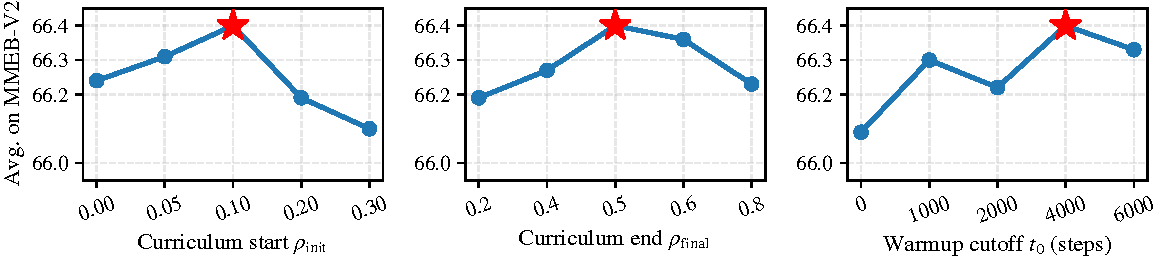
\includegraphics[width=0.9\textwidth]{figures/param_sweep_hns.pdf}
  \caption{Sensitivity to negative curriculum settings on MMEB-V2 (7B backbone).}
  \label{fig:param_hns}
\end{figure*}


